\subsection{OpenGL Pipeline}
\label{sec.opengl_pipeline}

In the OpenGL framework, the model and view transforms are combined in the \verb|GL_MODELVIEW| matrix. The 3D scene rendered by OpenGL must then be projected onto the computer screen using the \verb|GL_PROJECTION| matrix. In perspective projection, transforms a 3D point in a pyramid frustum in eye coordinates, truncated at the top, by the near plane $n$, and in the bottom, by the far plane $f$. The pyramid is bounded in $n$: in the horizontal by left and right coordinates, $l$ and $r$, and in the vertical by bottom and top coordinates, $b$ and $t$, respectively. The frustum is normalized in Normalized Device Coordinates (NDC), that is a mapping into a cube with the range of $x$-coordinate from $[l, r]$ to $[-1, 1]$, the y-coordinate from $[b, t]$ to $[-1, 1]$ and the $z$-coordinate from $[n, f]$ to $[-1, 1]$. The eye coordinates are defined in the left-handed coordinate system, but NDC uses the right-handed coordinate system. That is, the camera at the origin is looking along $-Z$ axis in eye space, but it is looking along $+Z$ axis in NDC. Since the OpenGL command glFrustum() accepts only positive values of near and far distances, they are negated during the construction of \verb|GL_PROJECTION| matrix.

\begin{figure}[h!]
\centering
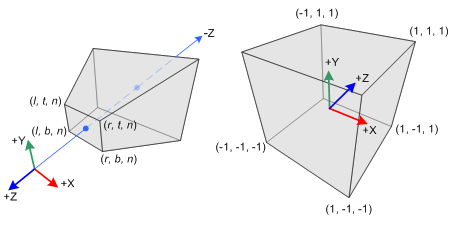
\includegraphics[width=0.9\linewidth,keepaspectratio=true]{figs/gl_projectionmatrix01.png}
\caption{Perspective Frustum and Normalized Device Coordinates (NDC)}
\label{fig.ndc}
\end{figure}

Part of the scene that is not going to be displayed, i.e., all vertex outside the frustum, is removed by frustum culling (clipping) and the edges of the polygon where clipping occurs are reconstructed. This is done transforming all vertex data from the eye coordinates, $(x_e, y_e, z_e)$, to the clip coordinate to clip coordinates $(x_c, y_c, z_c)$ in Equation~\ref{eq.clip}: 

\begin{equation}
\begin{aligned}
\begin{pmatrix} x_{c}\\y_{c}\\z_{c}\\w_{c} \end{pmatrix} &= 
M_{proj} \cdot \begin{pmatrix} x_{e}\\y_{e}\\z_{e}\\w_{e} \end{pmatrix}\\
%\begin{pmatrix} x_{ndc}\\y_{ndc}\\z_{ndc}\end{pmatrix} &=
%\begin{pmatrix} x_{c}/w_{c}\\y_{c}/w_{c}\\z_{c}/w_{c} \end{pmatrix}\\
\end{aligned}
\label{eq.clip}
\end{equation}

The clipping is performed in the clip coordinates by comparing with $w_c = -z_e$. If any clip coordinate is less than $-w_c$, or greater than $w_c$, then the vertex will be discarded. Then, those clip coordinates are also transformed to NDC by dividing the coordinates by the $w_c$ component in Equation~\ref{eq.ndc_coords}.
Bear in mind that both clipping and NDC transformations are integrated into \verb|GL_PROJECTION| matrix.

\begin{equation}
\begin{aligned}
\begin{pmatrix} x_{ndc}\\y_{ndc}\\z_{ndc}\end{pmatrix} &=
\begin{pmatrix} x_{c}/w_{c}\\y_{c}/w_{c}\\z_{c}/w_{c} \end{pmatrix}\\
\end{aligned}
\label{eq.ndc_coords}
\end{equation}

Then, a 3D point in eye space is projected onto the near plane. The following diagrams show how a point $(x_e, y_e, z_e)$ in eye space is projected to $(x_p, y_p, z_p)$ on the near plane.

\begin{figure}[h!]
\centering
\begin{tabular}{cc}
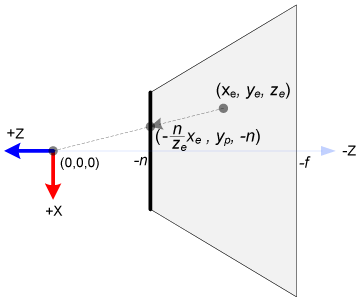
\includegraphics[width=0.45\linewidth,keepaspectratio=true]{figs/gl_projectionmatrix03.png}
&
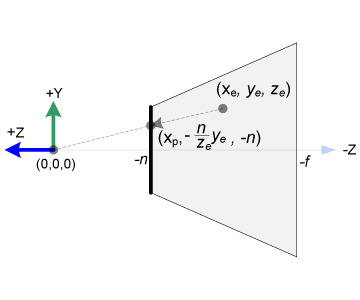
\includegraphics[width=0.45\linewidth,keepaspectratio=true]{figs/gl_projectionmatrix04.png}
\\
(a) Top View of Frustum
&
(b) Side View of Frustum
\end{tabular}
\label{fig.frustum}
\caption{Views of the frustum.}
\end{figure}

%From the top view of the frustum, the $x$-coordinate of eye space, $x_e$ is mapped to $x_p$, which is calculated by using the ratio of similar triangles;

%\begin{equation}
%\begin{aligned}
%\begin{split}
%\frac{x_p}{x_e}&=\frac{-n}{z_e}\\
%x_p&=\frac{-n \cdot x_e}{z_e}\\
%   &=\frac{n \cdot x_e}{-z_e}
%\end{split}
%\end{aligned}
%\label{eq.xp}
%\end{equation}

%From the side view of the frustum, $y_p$ is also calculated in a similar way; 

%\begin{equation}
%\begin{aligned}
%\begin{split}
%\frac{y_p}{y_e}&=\frac{-n}{z_e}\\
%y_p&=\frac{-n \cdot y_e}{z_e}\\
%   &=\frac{n \cdot y_e}{-z_e}
%\end{split}
%\end{aligned}
%\label{eq.yp}
%\end{equation}

Note that both $x_p$ and $y_p$ depend on $z_e$; they are inversely proportional to $-z_e$. In other words, they are both divided by $-z_e$. It is a very first clue to construct \verb|GL_PROJECTION| matrix. Therefore, the $w$-component of the clip coordinates is set as $-z_e$. And, the 4th row of \verb|GL_PROJECTION| matrix becomes $(0, 0, -1, 0)$: 

\begin{equation}
\begin{aligned}
\begin{split}
\begin{pmatrix} x_{c}\\y_{c}\\z_{c}\\w_{c} \end{pmatrix} &= 
\begin{pmatrix} 
\cdot & \cdot & \cdot & \cdot \\
\cdot & \cdot & \cdot & \cdot \\
\cdot & \cdot & \cdot & \cdot \\
0 & 0 & -1 & 0 \\
\end{pmatrix} &=
\begin{pmatrix} x_{e}\\y_{e}\\z_{e}\\w_{e} \end{pmatrix}
\end{split}
\end{aligned}
\label{eq.rows}
\end{equation}

%\begin{figure}[h!]
%\centering
%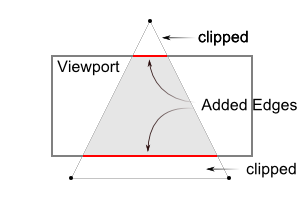
\includegraphics[width=0.9\linewidth,keepaspectratio=true]{figs/gl_frustumclip.png}
%\caption{A triangle clipped by frustum}
%\label{fig.clipping}
%\end{figure}

When all other entries in Equation~\ref{eq.rows} are obtained~\cite{schreiner2004}, the complete projection matrix is: 

\begin{equation}
\begin{aligned}
M_{proj} &= 
\begin{pmatrix} 
\frac{2n}{r-l} & 0 & \frac{r+l}{r-l} & 0 \\
0 & \frac{2n}{t-b} & \frac{t+b}{t-b} & 0 \\
0 & 0 & -\frac{f+n}{f-n} & -\frac{2fn}{f-n} \\
0 & 0 & -1 & 0 \\
\end{pmatrix} \\
\end{aligned}
\label{eq.projection_matrix}
\end{equation}


